%%%%%%%%%%%%%%%%%%%%%%%%%%%%%%%%%%%%%%%%%%%%%%%%%%%%%%%%%%%%%%%%%%%%%%%%%%%%%%%%

\talksection{Overview}

\begin{frame}{SPMD Vectorizer}

\begin{itemize}
    \item Is used to vectorize a SPMD program's entry point function
    \item Given a function $F$ and vectorization factor $N$, produces a function $VF_N$
    \begin{itemize}
        \item Calling $VF_N$ is like calling $F$, but $N$ times (on consecutive work-items)
        \item $F$ and $VF_N$ have the same signature
    \end{itemize}
    
    \item The original function can be preserved or not
    \begin{itemize}
        \item In-place: vectorize the original function, no need for cloning
        \item Transform cloned function: allow vectorization to fail
    \end{itemize}
    
    \item Vectorization may be allowed to fail
    \begin{itemize}
        \item On failure, the original function can be used 
    \end{itemize}
\end{itemize}

\end{frame}

%%%%%%%%%%%%%%%%%%%%%%%%%%%%%%%%%%%%%%%%%%%%%%%%%%%%%%%%%%%%%%%%%%%%%%%%%%%%%%%%

\begin{frame}{Structure}

\begin{itemize}
    \item Pipeline structure
    \begin{itemize}
        \item Function to vectorize is repeatedly transformed by different stages
        \item Stages are independent from each other
        \item Each stage consists of one or more IR passes
        \item Most stages require some analysis
    \end{itemize}
\end{itemize}

\center{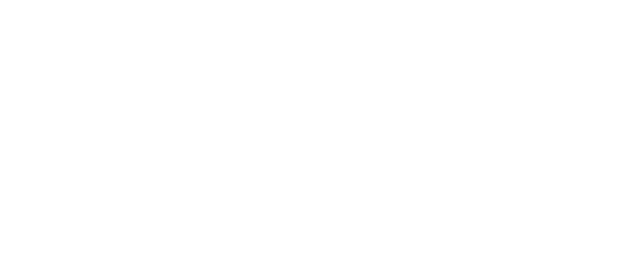
\includegraphics[width=0.8\textwidth]{images/stages.pdf}}

\end{frame}

%%%%%%%%%%%%%%%%%%%%%%%%%%%%%%%%%%%%%%%%%%%%%%%%%%%%%%%%%%%%%%%%%%%%%%%%%%%%%%%%

\begin{frame}{Analyses}

\begin{itemize}
    \item Capture information about the IR to vectorize
    \item May be invalidated after IR transformations
    \item May depend on other analyses
\end{itemize}

\end{frame}

%%%%%%%%%%%%%%%%%%%%%%%%%%%%%%%%%%%%%%%%%%%%%%%%%%%%%%%%%%%%%%%%%%%%%%%%%%%%%%%%

\begin{frame}{Analyses}

\begin{itemize}
    \item Uniform Value Analysis
    \begin{itemize}
        \item Marks values as either \uniform{uniform} or \varying{varying}
    \end{itemize}

    \item Control Flow Analysis
    \begin{itemize}
        \item Determines which basic blocks are \varying{divergent}
        \item Builds a Control Dependency Graph
    \end{itemize}
    
    \item SIMD Width Analysis
    \begin{itemize}
        \item Chooses a 'good' width $N$ based on register/instruction usage
    \end{itemize}
    
    \item ...
\end{itemize}

\end{frame}

%%%%%%%%%%%%%%%%%%%%%%%%%%%%%%%%%%%%%%%%%%%%%%%%%%%%%%%%%%%%%%%%%%%%%%%%%%%%%%%%

\begin{frame}{Implementation Level: IR or MI?}

\begin{itemize}
    \item IR Level
    \begin{itemize}
        \item (+) Use-def graph and RAUW make for straightforward transformations
        \item (+) Easy to target multiple platforms
        \item (?) Generally higher-level (simpler implementation?)
        \item (-) Platform-specific features more difficult to use
        \item (-) Predication only for select operations (select, load/stores)
    \end{itemize}

    \item MachineInstr level
    \begin{itemize}
        \item (+) Easy to use platform-specific features (e.g. predication, mask registers)
        \item (?) Generally lower-level (more powerful?)
        \item (-) More platform-specific code
        \item (-) Graph-based transformations not as straightforward
    \end{itemize}
    
\end{itemize}

\end{frame}

%%%%%%%%%%%%%%%%%%%%%%%%%%%%%%%%%%%%%%%%%%%%%%%%%%%%%%%%%%%%%%%%%%%%%%%%%%%%%%%%

%\begin{frame}{Implementation strategy}
%
%% TODO: Skip slide?
%\begin{itemize}
%    \item Create test kernels
%    \begin{itemize}
%        \item Start with very simple kernels (e.g. copy buffer, add two buffers)
%        \item Gradually add more features (e.g. non-sequential memory accesses, vector instructions, etc)
%    \end{itemize}
%
%    
%    \item Suggested implementation order
%    \begin{itemize}
%        \item Preparation and packetization first (required for simplest kernels)
%        \item Then easier features: builtins, memory addressing, scalarization, instantiation
%        \item More complex features last: control flow, optimizations
%    \end{itemize}
%\end{itemize}
%
%\end{frame}
